\section{Gradient SHAP}

Gradient SHAP (GradSHAP) was introduced by Erion et al. \cite{erion2019learning}\footnote{This paper is a preprint, it is still under the review at ICLR conference} and combined ideas from Integrated Gradients \cite{sundararajan2017axiomatic}, SHAP \cite{lundberg2017unified}, and SmoothGrad \cite{smilkov2017smoothgrad}. As mentioned in chapter \ref{section:ig}, IG has a problem with selecting the right baseline for specific a model. There were attempts to fix a problem with the baseline \cite{smilkov2017smoothgrad}\cite{fong2017interpretable}\cite{sturmfels2020visualizing} but selecting the right baseline with the "absence of feature" depends highly on the model architecture and datasets used in the training process.


\begin{equation}
    ExpectedGradients_{i}(x) ::= \int_{x'}\left( (x_{i} - x'_{i})\times\int_{\alpha=0}^1\frac{\partial F(x'+\alpha \times (x - x'))}{\partial x_i}{d\alpha} \right)p_D(x')\partial x'
    \label{eq:gradshap-full-eq}
\end{equation}

Erion et al. present an idea of \textit{expected gradients}, which tries to avoid specifying single $x'$ and use the data distribution instead $p_D$ (eq. \ref{eq:gradshap-full-eq}). Where $x$ is an input vector, $F$ is a model, $\alpha$ is an interpolation factor.


\begin{equation}
    ExpectedGradient^{expected}_{i}(x) ::= \underset{x' \sim D, \alpha \sim U(0,1)}{E} \left[(x_{i}-x'_{i})\times\frac{\partial F(x'+\alpha \times (x - x'))}{\partial x_i} \right]
    \label{eq:gradshap-aprox}
\end{equation}

As in the IG definition (eq. \ref{eq:ig-full-eq}), calculating the integral is not possible, two integrals in the Expected Gradients have the approximate value solution (eq. \ref{eq:gradshap-aprox}). Where $D$ is a our data and $\alpha$ comes from the uniform distribution $U(0,1)$.

\begin{wrapfigure}{L}{0.40\textwidth}
  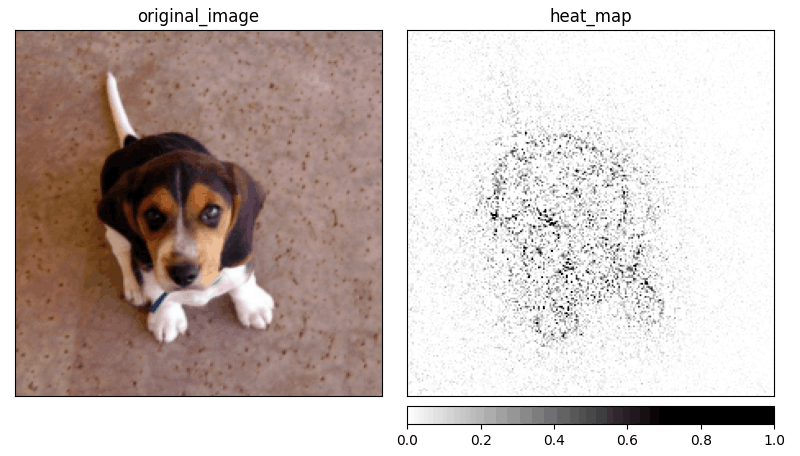
\includegraphics[width=0.40\textwidth]{methods/images/gradshap-beagle.png}
  \caption{Visualization of the saliency map by the GradSHAP generated for the class \textit{beagle}. The result is calculated with five random samples. Image source: \textit{Stanford Dogs} \cite{stanford-dogs}}\label{fig:gradshap-beagle}
  \vspace{1mm}
\end{wrapfigure}

In practice, this approach allows to approximate SHAP values. It computes expectations of gradients by sampling from the baselines and add noise to each input sample, $n$ times. GradSHAP assumes that input features are independent of each other and the explanation is simply a composition of individual features' contribution.

\vspace{\baselineskip}

In recent implementations \cite{kokhlikyan2020captum}, the method has multiple variants. One of the most important changes is to allow to replace $U(0,1)$ with the Gaussian distribution ${\mathcal {N}}(0 ,\sigma ^{2})$. Using a Gaussian distribution allows modifying the standard deviation $\sigma$ base on the original data. An example of the attribution generated by the GradSHAP method is shown in Figure \ref{fig:gradshap-beagle}.